\documentclass[10pt,journal,twocolumn,twoside]{IEEEtran}
\usepackage{amsmath,amssymb,amsfonts,float}
\usepackage{graphicx,bm,psfrag,amsmath,enumitem,amsthm}
\def\mmax{\mathop{\mbox{\scriptsize max}}}
\def\argmin{\mathop{\mbox{arg\,min}}}
\def\argmax{\mathop{\mbox{arg\,max}}}
\newcommand{\defequal}{\stackrel{\mathrm{def}}{=}}
\renewcommand{\vec}[1]{{\ensuremath{\boldsymbol{#1}}}}
\newcommand{\popt}{\ensuremath{P^{(K)}_{opt}}}
\pagestyle{plain}
\usepackage{algorithm, algorithmic}
\renewcommand{\algorithmicrequire}{ \textbf{Input:}} %Use Input in the format of Algorithm
\renewcommand{\algorithmicensure}{ \textbf{Procedures:}} %UseOutput in the format of Algorithm
\newtheorem{mypro}{Proposition}
% correct bad hyphenation here
%\hyphenation{op-tical net-works semi-conduc-tor}
\usepackage{CJK}
\usepackage{color}
\usepackage{url}
\usepackage{geometry}
\geometry{left=0.75in, right=0.73in, top=0.75in, bottom=0.75in}
%\def\BibTeX{{\rm B\kern-.05em{\sc i\kern-.025em b}\kern-.08em
%    T\kern-.1667em\lower.7ex\hbox{E}\kern-.125emX}}

\begin{document}

\title{Joint Precoding and Power Allocation for Hybrid Precoding Systems via Rank-Constrained D.C. Programming}
\author{\IEEEauthorblockN{Guanchong Niu, Qi Cao, Man-On Pun\IEEEauthorrefmark{3}\\
		\IEEEauthorblockA{Shool of Science and Engineering,\\
			The Chinese University of Hong Kong, Shenzhen\\
			Guangdong, China, 518172
			\thanks{This work was supported, in part, by the Shenzhen Science and Technology Innovation Committee under Grant No. ZDSYS20170725140921348, the Robotic Discipline Development Fund (2016-1418) from the Shenzhen Government and the National Natural Science Foundation of China under Grant No. 61731018.} \thanks{\IEEEauthorrefmark{3} Corresponding author, email: SimonPun@cuhk.edu.cn.}
}}}
\maketitle\thispagestyle{plain}\pagestyle{plain}

\begin{abstract}
Hybrid analog and digital precoding has recently been proposed for massive multiple-input multiple-output (MIMO) systems. However, it is challenging to optimize the design of precoding and power allocation as the optimization problem is highly non-convex. In this work, the non-convex problem is cast into the D.C. (difference of two convex functions) programming framework. To cope with the high dimensionality of the problem, an iterative rank-constrained D.C. programming technique is developed. As a result, the proposed algorithm is capable of directly maximizing the weighted sum-rate (WSR) of each user to take in account the quality of service (QoS) requirement. Furthermore, the monotonic convergence behavior of the proposed iterative algorithm is proved. Finally, simulation results confirm the effectiveness of the proposed iterative algorithm.
\end{abstract}

%\begin{keywords}
%BDMA, Hybrid Beamforming, Block Diagonal Precoder, PAPR, User Scheduling.
%\end{keywords}

\begin{IEEEkeywords}
	Massive MIMO, Hybrid Beamforming, D.C. Programming, Power Allocation.
\end{IEEEkeywords}

%\titlepgskip=-15pt

%\maketitle

\section{Introduction}\label{sec:introduction}
To meet the ever-increasing demand for higher user data rates, it is envisioned that the next-generation cellular systems will be equipped with massive antenna arrays \cite{molisch2005capacity}. Capitalizing on a large number of antennas at the base station (BS), BDMA was first proposed to decompose the multiuser multiple-input multiple-output (MU-MIMO) system into multiple single-user MIMO channels by multiplexing multiple users' data onto non-overlapping beams in \cite{sun2015beam}. BDMA is particularly attractive in practice as beamforming is commonly implemented in the analog domain using low-cost phase shifters. Meanwhile, to eliminate the multiuser interference while avoiding the unaffordable hardware cost and power consumption of full digital beamforming, hybrid digital and analog beamforming has been proposed for massive MIMO transmissions by dividing the precoding process into two steps, namely analog and digital precoding \cite{alkhateeb2014channel}. More specifically, the transmitted signals are first precoded digitally using a smaller number of RF chains followed by the analog precoding implemented with a much larger number of low-cost phase shifters. As a result, the hybrid analog-digital precoding architecture requires significantly less RF chains as compared to the fully digital precoding.

Despite its many advantages, the analog and digital beamforming requires highly computational design of the analog and digital precoding vectors. In addition, power allocation design plays an important role in managing co-channel interference in multiuser (MU) networks. However, joint precoding and power allocation design is usually highly non-convex as these precoding and power constraints are coupled. To the authors' best knowledge, no closed-form solutions to the joint precoding and power allocation design have been reported in the literature. Instead, most existing works separate the precoding and power allocation problem to two isolated problems. For instance, \cite{sohrabi2016hybrid} alternatively optimizes the power allocation for the sum-rate capacity maximization problem implementing water filling by assuming the analog precoders are strictly orthogonal among distinct users. For single antenna transceivers, the difference of two convex functions (D.C.) programming algorithm is presented to maximize the weighted sum-rate (WSR) by finding the optimal power allocation in \cite{kha2012fast}. It is worth noting that most exiting works approximate the sum-rate maximization problem with an interference minimization (e.g. zero-forcing) problem.

Finally, for multi-user wireless networks, it is highly desirable to design a system that satisfies the quality of service (QoS) constraint for each user. In the literature, such QoS requirements are commonly met by adjusting the power allocated to different users in the system \cite{palomar2004optimum}. For instance, the signal-to-interference ratio (SIR) or signal-to-interference-and-noise ratio (SINR)-balancing schemes are proposed for multiuser code division multiple access (CDMA) systems by allocating power on each data stream.\cite{xie2017sinr}. The resulting system satisfies the QoS requirement as all users have the same SIR/SINR value. However,  such balanced SIR/SINR approaches imply that the system performances is limited by the worst user, which incurs performance degradation in terms of overall system sum-rate capacity.

\begin{figure*}[ht]
	\begin{center}
		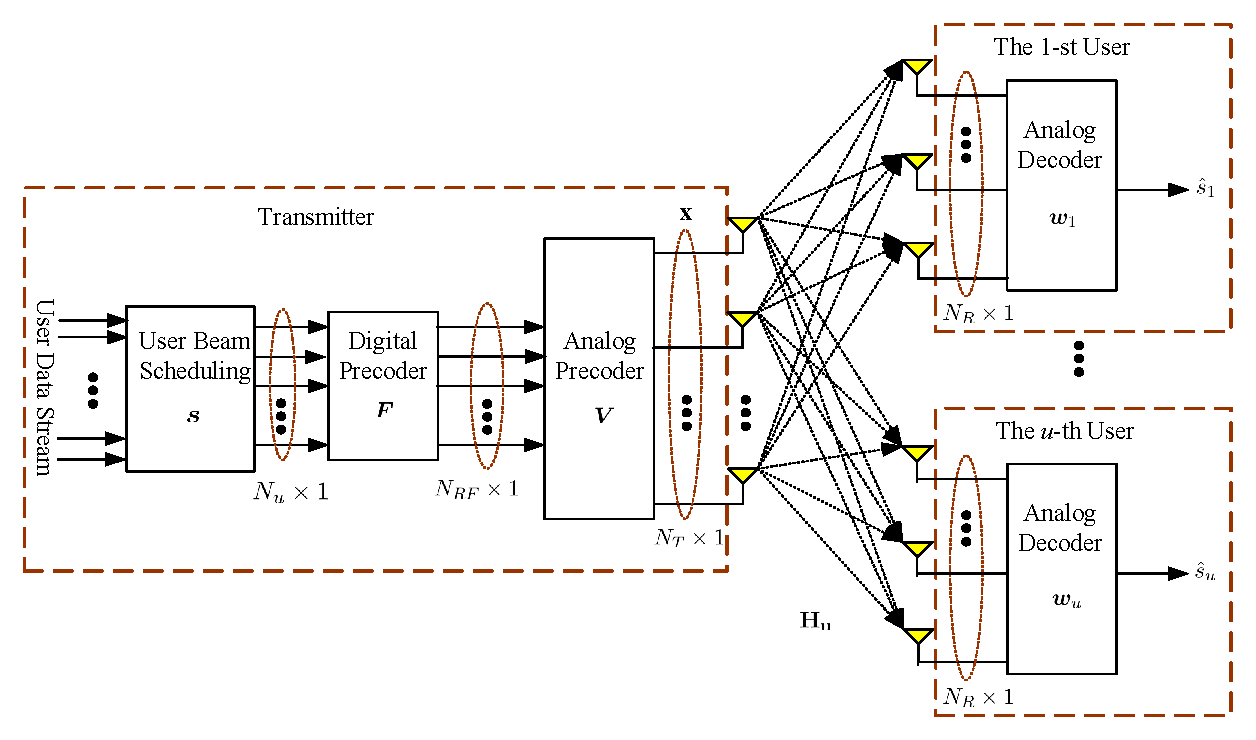
\includegraphics[scale=0.6]{Figure/SystemSchematic_new.pdf}
		\caption{Block diagram of the hybrid precoding system under consideration.}\label{fig:BlockDiagram}
	\end{center}
\end{figure*}


Motivated by the aforementioned challenges, this work develops joint precoding and power allocation for hybrid precoding systems using the rank-constrained D.C. programming. The main contributions of this work are summarized as follows:

\begin{itemize}[leftmargin=*]
		
\item In sharp contrast to the conventional optimization algorithms that separate the precoding and power allocation problems independently, a rank-constrained D.C. problem is presented to jointly optimize the digital precoder and power allocation to different data streams;

\item To solve the general rank-constrained D.C. problems, an iterative algorithm is proposed to formulate the objective function as a standard convex optimization problem in each iteration. The convergence of the proposed algorithm is proved.

\item Finally, we apply the newly established iterative ank-constrained D.C. programming technique to maximize the WSR with QoS constraints for each user by jointly optimizing the precoder design and power allocation. Simulation results are shown to demonstrate the effectiveness of the proposed algorithm.

\end{itemize}


{\underline{Notation}: In this paper, we use uppercase boldface letters to denote matrices and lowercase boldface letters to denote vectors. $j = \sqrt{-1}$ and $\bm{I}_N$ denotes the identity matrix with size $N\times N$. ${\bm A}^T$ and ${\bm A}^H$ denote transpose and conjugate transpose of ${\bm A}$, respectively. $[\bm{a}]_{i}$ denotes the $i$-element of ${\bm a}$. $\|\bm{A}\| $ stands for the L2 norm of ${\bm A}$ while $|A|$ denotes the absolute value of $A$.  $\textbf{rank}(\bm{A})$ and $\textbf{trace}(\bm{A})$ represent the rank and trace of $\bm{A}$, respectively. Finally, $\bigtriangledown f(\bm{A})$ represents the gradient of function $f(\bm{A})$.}

%\begin{figure*}[ht]
%	\begin{center}
%		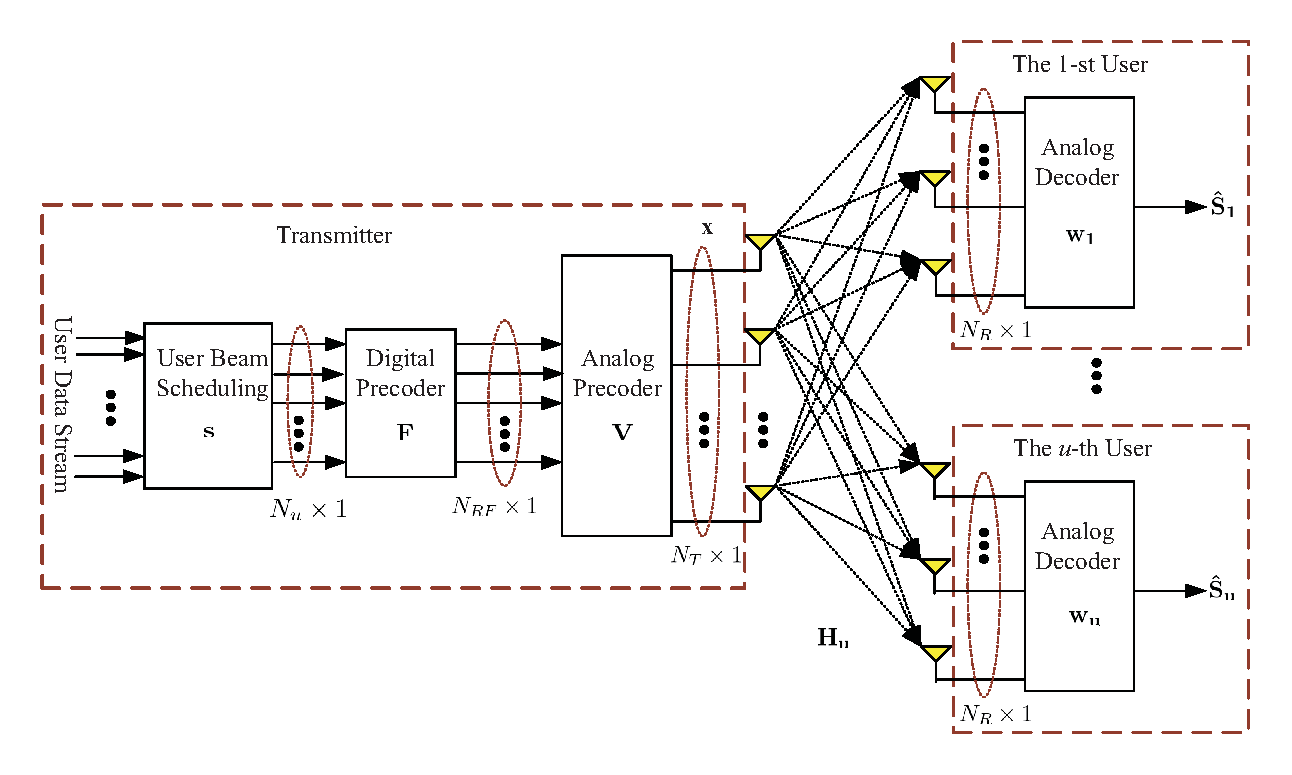
\includegraphics[scale=0.6]{Figure/SystemSchematic_new.eps}
%		\caption{Block diagram of the hybrid precoding system under consideration.}\label{fig:BlockDiagram}
%	\end{center}
%\end{figure*}

%\section*{References and Footnotes}

\section{System model and problem formulation}\label{system}



\subsection{System Model}

We consider a multiuser mmWave MIMO system shown in \figurename{ \ref{fig:BlockDiagram}}, in which a transmitter equipped with $N_{RF}$ RF chains and $N_T$ antennas transmits $N_U$ data streams to $N_U$ receivers with $N_R$ receive antennas. Following the same assumption commonly employed in the literature \cite{alkhateeb2015limited}, we assume only one data stream is designated to each scheduled receiver. We use ${\bm s}(n)$ to denote the $n$-th block of $N_U$ data to be transmitted with $\mathbb{E}\left[\bm{ss}^H\right]=\frac{1}{N_U}\bm{I}_{N_U}$. In the sequel, we concentrate on a single block and omit the temporal index $n$ for notational simplicity.


The hybrid precoding system first multiplies ${\bm s}$ with the digital precoding matrix $\bm{F}=\left[{\bm f}_1,{\bm f}_2,\cdots, {\bm f}_{N_U}\right]$ with ${\bm f}_u$ of dimension $N_{RF}\times 1$ being the digital beamforming vector for the $u$-th user, $u=1,2,\cdots,N_U$. After that, the output signal will be multiplied by the analog precoding matrix $\bm{V}=\left[{\bm v}_1,\cdots,{\bm v}_u,\cdots,{\bm v}_{N_{RF}}\right]$ with ${\bm v}_u$ of dimension $N_T\times 1$ being the $u$-th analog beamforming vector for $u = 1,2,\cdots,N_{RF}$. The resulting precoded signal $\bm x$ of dimension $N_T\times 1$  can be expressed as

\begin{equation}{\label{eq:transx1}}
{\bm x} = \bm{V}\cdot \bm{F}\cdot\bm{s}= \bm{V}\sum_{u=1}^{N_U}\bm{f}_u s_u.
\end{equation}

The precoded signal $\bm x$ is then broadcast to $N_U$ users. The signal received by the $u$-th user is given by

\begin{eqnarray}{\label{eq:transx2}}
{\bm y}_u &=& \bm{H}_u \bm{x} + \bm{n}_u\\
&=&\bm{H}_u \bm{V}\bm{f}_us_u+\bm{H}_u \bm{V}\sum_{\substack{i=1 \\ i\neq u}}^{N_U}\bm{f}_is_i+\bm{n}_u,
\end{eqnarray}
where $\bm{H}_u$$\in\mathbb{C}^{N_R\times N_T}$ is the MIMO channel matrix between the transmitter and the $u$-th receiver\cite{el2014spatially}. Furthermore, $\bm{n}_u$ is complex additive white Gaussian noise with zero mean and variance equal to $\sigma_u^2$.

Assuming the receivers are all low-cost terminals that perform analog beamforming only in decoding, the decoded signal by the $u$-th user denoted by $\hat{s}_u$ is given by
\begin{equation}{\label{eq:hats}}
\hat{s}_u = \bm{w}_u^H \bm{H}_u \bm{V} \bm{f}_{u} \bm{s} + \bm{w}_u^H \bm{\tilde{n}}_u,
\end{equation}
where ${\bm w}_u$ of dimension $N_R\times 1$ is the analog beamforming vector employed by the $u$-th receiver with the power constraint of $\|\bm{w}_u\|^2=1$ and
\begin{equation}
\bm{\tilde{n}}_u=\bm{H}_u \bm{V}\sum_{\substack{i=1 \\ i\neq u}}^{N_U}\bm{f}_is_i+\bm{n}_u.
\end{equation}
Note that the first term in Eq.~(\ref{eq:hats}) stands for the desired signal while the second term is the sum of its own receiver noise and interference from other users.

\subsection{Channel Model}
As shown in \cite{rappaport2014millimeter}, the mmWave wireless channel can be well modeled by the Saleh-Valenzuela model. Following the same approach developed in \cite{alkhateeb2015limited}, we assume that each scatter only contributes one single propagation path. As a result, the $u$-th user's channel model can been modeled as
\begin{equation}{\label{eq:Hu}}
\bm{H}_u = \sqrt{\frac{N_{T}N_{R}}{L_{u}}}\sum_{l=1}^{L_u}\alpha_{u,l}\cdot \bm{a}_{R}(\phi^r_{u,l},\theta^r_{u,l}) \cdot\bm{a}_{T}^{H}(\phi^t_{u,l},\theta^t_{u,l}),
\end{equation}
where $L_u$ is the number of scatters of the $u$-th user's channel. Furthermore, $\alpha_{u,l}$, $\theta^r_{u,l}/\phi^r_{u,l}$ and $\theta^t_{u,l}/\phi^t_{u,l}$ are the complex path gain, azimuth/elevation angles of arrival(AoA) and azimuth/elevation angles of departure(AoD) of the $l$-th path of the $u$-th user, respectively. Finally, ${\bm a}$ is the array response vector. For an uniform planar array (UPA) of size $W\times Q$ considered in this work, the array response vector ${\bm a}$ is given by
\begin{flalign}\label{eq:UPAvec1}
\bm{a}(\phi,\theta) =&\frac{1}{\sqrt{WQ}}\left[1,  e^{j\kappa d(\sin\phi \sin\theta +\cos\theta)},   \right. &&\nonumber\\
&\left. \cdots, e^{j\kappa d\left((P-1)\sin\phi \sin\theta +(Q-1)\cos\theta\right)}\right]^T,&&
\end{flalign}
where $\kappa =\frac{2\pi}{\lambda}$ is the wavenumber and $d$ is the distance between two adjacent antennas.


\subsection{Problem Formulation}
For notational simplicity, we denote by ${\bm{g}}_{u}^H$ the effective array gain of the $u$-th user with
\begin{equation}\label{eq:defgu}
{\bm{g}}_{u}^H = \bm{w}^H_u \bm{H}_u \bm{V}.
\end{equation}

Then, the channel capacity of the $u$-th user is given by
\begin{equation}\label{eq:6}
R_u(\bm{p},\bm{W},\bm{V}, \bm{F}) = \log\left(1+\frac{p_u|{\bm{g}}_{u}^H \bm{f}_u|^2}{\sum_{\substack{i=1 \\ i\neq u}}^{N_U}p_i|{\bm{g}}_{u}^H\bm{f}_i|^2+\sigma_u^2}\right).
\end{equation}

Subsequently, the system WSR can be formulated as
\begin{equation}
R_{tot}=\sum_{u=1}^{N_U} \tau_uR_u(\bm{p},\bm{W},\bm{V}, \bm{F}),
\end{equation}
where $\bm{\tau} = \left[\tau_1, \tau_2, \cdots, \tau_{_{N_U}}\right]$ with $\sum^{N_U}_{u = 1} \tau_u= N_U$ are the corresponding weights for users and $\bm{p} = [p_1, p_2, \cdots, p_{_{N_U}}]$.

Finally, the optimal design of the digital and analog precoding matrices as well as power allocation can be formulated as
\begin{align}\label{eq:maxsumrate}
\mathcal{P}_1: \quad&\underset{\bm W, \bm{V},\bm F}{\text{maximize}}\quad R_{tot}(\bm{p},\bm{W}, \bm{V}, \bm{F})\\
\text{subject to} \quad&C_1: | [\bm{v}_{u}]_i |^2=1/N_T,\quad 0<i\leq N_T; \nonumber\\
&C_2: |[\bm{w}_{u}]_j|^2=1/N_R, \quad  0<j \leq N_R;\nonumber\\
&C_3: \|\bm{V} \bm{f}_u\|^2 = 1, \quad 0<u<N_U;\nonumber\\
&C_4: \sum_{u=1}^{N_U}p_{u} \leq P;\nonumber\\
&C_5: R_{u}\geq \lambda_{u}, \quad 0<u<N_U, \nonumber
\end{align}
where $C_1$ and $C_2$ are the analog constraints for receiver and transmitter. $C_3$ ensures that each RF chain is of unit power. The total transmitter power is constrained by $P$ as shown in $C_4$. Finally, $C_5$ ensures that the $u$-th user's capacity should be guaranteed not less than a certain threshold $\lambda_{u}$.

Since the problem $\mathcal{P}_1$ is highly non-convex, it is analytically intractable to derive a closed-form solution to $\mathcal{P}_1$. In this paper, we first design the analog precoder to relax the phase constraints. After that, a general rank-constrained D.C. programming technique is proposed to derive the optimal digital precoder and power allocation by transforming the problem in each iteration as a standard convex optimization problem.

\section{Analog Beamforming Design}\label{analog}

We begin with the analog beamforming design for both transmitter and receiver. It is well-known that distinct array response vectors are asymptotically orthogonal as the number of antennas in an antenna array goes to infinity \cite{sun2015beam}, {\em i.e.}
\begin{equation}\label{Eq:assumption}
\lim_{N\rightarrow +\infty} \bm{a}^{H}(\phi^t_{k,u},\theta^t_{k,u}) \cdot\bm{a}(\phi^t_{\ell,v},\theta^t_{\ell,v})=\delta(k-\ell)\delta(u-v).
\end{equation}
However, since the antenna number is finite in practice, the residual interference must be considered in the analog precoding design. Recalling the channel model presented in Equation~(\ref{eq:Hu}), we can asymptotically orthogonalize the transmitted signals by optimizing the design of $\bm{{w}}_{u}$ and $\bm{{v}}_{u}$:
\begin{align}\label{eq:group-scheduling}
\{\bm{{w}}^*_{u}, \bm{{v}}^*_{u}\} &=\underset{\tilde{\bm w }_{u}, \tilde{\bm v}_{u}}{\argmax}
\sum_{u=1}^{M_k}\log\left(1+ \text{SINR}\left(\tilde{\bm w}_{u}, \tilde{\bm v}_{u}\right)\right)  \\ \nonumber
\text{subject to}&\quad \tilde{\bm v}_{u}\in \mathcal{A}^t_{u};\\
&\quad \tilde{\bm w}_{u}\in \mathcal{A}^r_{u}, \nonumber
\end{align}
where the array response vectors in transmitter and receiver are denoted by
\begin{align}
\mathcal{A}^t_{u} = \left[\bm{a}_{T}(\phi^t_{{u,1}},\theta^t_{{u,1}}),\cdots,\bm{a}_{T}(\phi^t_{{u,L_{u}}},\theta^t_{{u,L_{u}}})\right],
\nonumber \\
\mathcal{A}^r_{u} = \left[\bm{a}_{R}(\phi^r_{{u,1}},\theta^r_{{u,1}}),\cdots,\bm{a}_{R}(\phi^r_{{u,L_{u}}},\theta^r_{{u,L_{u}}})\right].
\end{align}

Furthermore, $\text{SINR}\left(\tilde{\bm w}_{u}, \tilde{\bm v}_{u}\right)$ is given by
\begin{equation}\label{SINR}
\text{SINR}_u\left(\tilde{\bm w}_{u}, \tilde{\bm v}_{u}\right) = \frac{|\tilde{\bm w}^H_{u} \bm{H}_{u} \tilde{\bm v}_{u}|^2}{\displaystyle\sum_{i=1,i\neq u}^{N_U}|\tilde{\bm w}^H_{u} \bm{H}_{u}\tilde{\bm {v}}_i|^2 + {1 \over \gamma} },
\end{equation}
where $\gamma = \frac{P}{N_{_U}\sigma_{u}^2}$ is the uniform SNR for each user and we have assumed that $\bm{f}_u\bm{f}_u^H = \bm{I}_{N_U}$. {\bf Simon: Why?}


The optimal analog precoder can be straightforwardly found by  exhaustively searching in the feasible sets of $\mathcal{A}^T_{k,u}$ and $\mathcal{A}^R_{k,u}$.

%The denominator in Eq. \eqref{SINR} only contains the inter-cluster interference since we assume that the intra-cluster interference can be  eliminated by digital precoder described in Section \ref{digital}. As a result, the inter-user interference can be asymptotically eliminated if a large number of beamforming antennas is employed. {\bf Simon: If inter-user interference can be asymptotically eliminated as $N\rightarrow +\infty$, the same conclusion can be also applied to the intra-cluster interference.}

%Using the analog beamforming vector in Eq.~(\ref{eq:group-scheduling}), the equivalent channel from the transmitter to user $u$ in cluster $k$ becomes $\bm{H}_{k,u}\bm{v}_{k,u}=\sqrt{N_{T}N_{R}}\alpha_{k,u}\cdot \bm{a}_{R}(\phi^r_{k,u},\theta^r_{k,u})$ and the equivalent channels to other users are all equal to zero vectors. Subsequently, the maximum ratio combing (MRC) is employed at the receiver and the resulting receive analog beamforming vector is given by:
%\begin{equation}
%\bm{w}^H_{k,u,l}=\bm{a}_{R}^{H}(\phi^r_{k,u,l},\theta^r_{k,u,l}).\\
%\label{eq:wku}
%\end{equation}

\section{Proposed rank-constrained d.c.  problem}\label{analogAndDigital}

For given analog precoders, we will derive the optimal digital precoder and power allocation in this section. Recalling the problem $\mathcal{P}_1$, the function of $R_{tot}(\bm{F}, \bm{p})$ is still non-convex.  To settle this challenge, we form the digital precoder as
\begin{equation}
\bar{\bm{F}}_{u} = p_u\bm{f}_{u} \bm{f}_{u}^H,
\end{equation}
with constraints $\textbf{rank}(\bar{\bm{F}}_{u})\leq 1$ and $\bar{\bm{F}}_{u} \succeq \bm{0}$. Denote by $\bm{\mathcal{F}} = [\bar{\bm{F}}^{(n)}_1, \bar{\bm{F}}^{(n)}_2,\cdots, \bar{\bm{F}}^{(n)}_{N_U}]$.

 Furthermore, the constraints $C_3$ and $C_4$ in $\mathcal{P}_1$ can be transformed as
\begin{equation}
 \sum_{u=1}^{N_U} p_u\|\bm{V} \bm{f}_{u}\|^2 = \sum_{u=1}^{N_U}\bm{V} \bar{\bm{F}}_u\bm{V} ^H \leq P.
\end{equation}

It is worth noting that the optimal digital precoder $\bm{f}_{u}^*$ is the eigenvector corresponding to the only one non-zero eigenvalue $p^*_u$ of optimal $\bar{\bm{F}}_u^*$, where $p^*_u$ is the optimal power allocation.

Then the Equation \eqref{eq:6} can be rewritten as
\begin{align}\label{eq:newR}
R_u(\bar{\bm{F}}_u) =& \log_2\left(1+\frac{\bm{g}_{u}^H \bar{\bm{F}}_u\bm{g}_{u}}{\sum_{\substack{i=1 \\ i\neq u}}^{N_U}{\bm{g}}_{u}^H\bar{\bm{F}}_i\bm{g}_u+\sigma_u^2}\right)\nonumber\\
=&\log_2\left(\sum_{i=1}^{N_U}\bm{g}_{u}^H \bar{\bm{F}}_i\bm{g}_{u} + \sigma_u^2\right) \nonumber\\
&\qquad -\log_2\left(\sum_{\substack{i=1 \\ i\neq u}}^{N_U}{\bm{g}}_{u}^H\bar{\bm{F}}_i\bm{g}_u+\sigma_u^2 \right).
\end{align}

Thereby the problem $\mathcal{P}_1$ can be reformulated as a D.C. problem with a rank constraint:
\begin{align}\label{eq:maxR}
\mathcal{P}_2: \quad&\underset{\bar{\bm{F}}}{\text{maximize}}\quad f(\bm{\mathcal{F}}) - g(\bm{\mathcal{F}})\\ \nonumber
\text{subject to} \quad&C_1: \sum_{u=1}^{N_U}\bm{V}^H \bar{\bm{F}}_u\bm{V} \leq P;\nonumber\\
&C_2: R_{u}\geq \lambda_{u}, u = 1,2,\cdots, N_U;\nonumber\\
&C_3: \bar{\bm{F}}_{u} \succeq \bm{0}, u = 1,2,\cdots, N_U; \nonumber\\
&C_4: \textbf{rank}(\bm{\bar{F}}_{u})\leq 1, u = 1,2,\cdots, N_U, \nonumber
\end{align}
where
\begin{align}
	f(\bm{\mathcal{F}}) = \sum_{u=1}^{N_U}\tau_u\log_2\left(\sum_{i=1}^{N_U}\bm{g}_{u}^H \bar{\bm{F}}_i\bm{g}_{u} + \sigma_u^2\right),\\
    g(\bm{\mathcal{F}}) = \sum_{u=1}^{N_U}\tau_u \log_2\left(\sum_{\substack{i=1 \\ i\neq u}}^{N_U}{\bm{g}}_{u}^H\bar{\bm{F}}_i\bm{g}_u+\sigma_u^2 \right).
\end{align}
It is worth noting that the QoS constraint $C_2$ can be straightforwardly reformulated as a convex constraint by the following transformation:
\begin{equation}
	\bm{g}_{u}^H \bar{\bm{F}}_u\bm{g}_{u} + (1-2^{\lambda_{u}}) \left( \sum_{\substack{i=1 \\ i\neq u}}^{N_U} \bm{g}_{u}^H \bar{\bm{F}}_i\bm{g}_{u} + \sigma_u^2 \right) \geq 0.
\end{equation}
Finally, a standard D.C programming problem is derived after dropping $C_4$. Next, the iterative algorithm will be given to solve the problem $\mathcal{P}_2$ by ignoring $C_4$ constraint.

Since the problem $\mathcal{P}_2$ still has high computational complexity, the optimal $\bm{\mathcal{F}}^*$ can be obtained by iteratively solving $\bar{\bm{F}}_u$ for $u = 1,2,\cdots, N_U$ until no improvement for next iteration as detailed in next section.

Similar to the procedures in \cite{kha2012fast}, the iterative algorithm gives the optimal $\bar{\bm{F}}_u^{(n+1)}$ at $n$-th iteration by solving the following convex problem:
\begin{align}\label{DC}
\underset{\bar{\bm{F}}_u}{\text{maximize}}&\quad f(\bar{\bm{F}}_u) - g(\bar{\bm{F}}^{(n)}_u) - \langle \bigtriangledown g(\bar{\bm{F}}^{(n)}_u), \bar{\bm{F}}_u -  \bar{\bm{F}}_u^{(n)} \rangle\\ \nonumber
\text{subject to}& \quad C_1, C_2, C_3\quad \text{in} \quad \mathcal{P}_2,
\end{align}
where $\langle \cdot \rangle$ denotes the inner product of two matrices, \textit{i.e.} $\langle \bm{A}, \bm{B} \rangle = \textbf{trace}(\bm{A}^T \bm{B})$. The gradient of $g(\bar{\bm{F}}^{(n)})$ is easily given by
\begin{equation}
	\bigtriangledown g(\bar{\bm{F}}^{(n)}_u) = \sum_{\substack{j=1 \\ j\neq u}}^{N_U}\frac{w_j/\ln 2}{\sum_{\substack{i=1 \\ i\neq j}}^{N_U} \bm{g}_{u}^H \bar{\bm{F}}_i\bm{g}_{u} +\sigma^2_j} \bm{g}_{j} \bm{g}_{j}^H.
\end{equation}
It is worth noting that $\langle \bigtriangledown g(\bar{\bm{F}}^{(n)}_u), \bar{\bm{F}}_u -  \bar{\bm{F}}_u^{(n)} \rangle$ is a real value since $\bigtriangledown g(\bar{\bm{F}}^{(n)}_u)$ and $\bar{\bm{F}}_u -  \bar{\bm{F}}_u^{(n)}$ are both hermitian.

\section{Proposed iterative algorithm for Rank-constrained D.C. problem}

To solve the problem $\mathcal{P}_2$, we will first introduce a rank constrained optimization problem (RCOP). Inspired by the RCOP, we propose an iterative algorithm to solve $\mathcal{P}_2$ by formulating a convex optimization problem in each iteration.
\subsection{The General RCOP}
We now consider the rank constraint $C_4$ in $\mathcal{P}_2$. A general RCOP to optimize a convex objective subject to a set of convex and rank constraints can be formulated as follows:
\begin{align}\label{eq:RCOP}
\mathcal{P}_3: \quad& \underset{\bm{X}}{\text{minimize}}   \quad f(\bm{X}) \\
\text{subject to}& \quad \bm{X} \succeq 0;\nonumber\\
& \quad \bm{X} \in \mathcal{C}; \nonumber\\
& \quad \textbf{rank}(\bm{X})\leq r, \nonumber
\end{align}
where $f(\bm{X})$ is a convex function, $\mathcal{C}$ is the set of given convex constraints and $\bm{X}\in \mathbb{C}^{m\times m}$ is a general positive semidefinite matrix.

The RCOP can be solved by an iterative method by gradually approaching the constrained rank \cite{sun2017rank}. At each iteration $n$, we will solve the following semidefinite programming (SDP) problem:
\begin{align} \label{rank}
\underset{\bm{X}^{(n+1)}, e^{(n)}}{\text{minimize}}  & \quad f(\bm{X}^{(n+1)})  + w e^{(n+1)} \\
\text{subject to}& \quad \bm{X}^{(n+1)} \succeq \bm{0};\nonumber\\
& \quad \bm{X}^{(n+1)}\in \mathcal{C}; \nonumber\\
&\quad e^{(n+1)}\bm{I}_{m-r} - \bm{U}^{(n)H} \bm{X}^{(n+1)} \bm{U}^{(n)} \succeq \bm{0};\nonumber\\
&\quad e^{(n+1)} \leq e^{(n)},\nonumber
\end{align}
where $w > 0$ is the weighting factor. Using eigenvalue decomposition (EVD), $\bm{U}^{n} \in \mathbb{C}^{{m}\times (m-r)}$ is the orthonormal eigenvectors corresponding to the $n-r$ smallest eigenvalues of $\bm{X}^{(n)}$ solved at previous $n$-th iteration. At the first iteration where $n=0$, $e^{(0)}$ is the $(m-r)$-th smallest eigenvalue of $\bm{X}^{(0)}$. $\bm{X}^{(0)}$ is obtained via
\begin{align} \label{x0}
\underset{{\bm{X}^{(0)}}}{\text{minimize}} & \quad f(\bm{X}^{(0)}) \\
\text{subject to}& \quad \bm{X}^{(0)} \succeq 0;\nonumber\\
& \quad \bm{X}^{(0)}\in \mathcal{C}, \nonumber
\end{align}
and $\bm{U}^{(0)}$ is the eigenvectors corresponding to $n-r$ smallest eigenvalues of $\bm{X}^{(0)}$.


\subsection{Iterative Algorithm for $\mathcal{P}_2$}
As shown in Section \ref{analogAndDigital}, Equation \eqref{DC} is obviously a concave optimization problem.
By combining the $\mathcal{P}_2$ and $\mathcal{P}_3$, an iterative algorithm for the rank-constrained D.C programming problem is derived.
The optimal $g(\bar{\bm{F}}^{(n+1)})$ in the $n$-th iteration is given by solving the following convex problem:
\begin{align} \label{rankconstrainedDC}
\underset{\bar{\bm{F}}_u, e^{(n+1)}}{\text{minimize}}  & \quad  t(\bar{\bm{F}}_u, e^{(n+1)}) \\
\text{subject to}&\quad \sum_{u=1}^{N_U}\bm{V}^H \bar{\bm{F}}_u\bm{V} \leq N_U;\nonumber\\
& \quad R_{u}\geq \lambda_{u}, u = 1,2,\cdots, N_U;\nonumber\\
&\quad \bar{\bm{F}}_u \succeq \bm{0};\nonumber\\
&\quad e^{(n+1)}\bm{I}_{N_U-1} - \bm{U}^{(n)H} \bar{\bm{F}}_u \bm{U}^{(n)} \succeq \bm{0};\nonumber\\
&\quad e^{(n+1)} \leq e^{(n)},\nonumber
\end{align}
where
\begin{align}
 &t(\bar{\bm{F}}_u, e^{(n+1)})\nonumber\\
  = &g(\bar{\bm{F}}^{(n)}_u) + \langle \bigtriangledown g(\bar{\bm{F}}^{(n)}_u), \bar{\bm{F}}_u -  \bar{\bm{F}}_u^{(n)} \rangle  -  f(\bar{\bm{F}}_u) + w e^{(n+1)},\nonumber
\end{align}

 and $\bm{U}^{(n)}$ is the eigenvectors corresponding to $N_U-1$ smallest eigenvalues of  $\bar{\bm{F}}^{(n)}_u$.

Despite the formidable appearance of Equation \eqref{rankconstrainedDC}, it is indeed a standard convex optimization problem that can be solved via available convex software packages, such as CVX \cite{cvx}.

The proposed iterative algorithm can be summarized as \textbf{Algorithm 1}. In each iteration, we solve a D.C programming problem and update the optimal $\bar{\bm{F}}^{*(n)}_u$. If the WSR $s^{(n)}$ can be no longer improved, the digital precoder $\bar{\bm{F}}^{(n)}_{u+1}$ of $(u+1)$-th user is then optimized successively. The iteration will stop if no any improvement for $ t(\bar{\bm{F}}^{(n)}_{u})$.

\begin{algorithm}[h] 		
	\caption{Proposed Iterative Algorithm for Rank-constrained D.C. Problem}
	\label{beam_cluster}
	\begin{algorithmic}
		\REQUIRE  \quad
		\STATE Effective channel: $\bm{g}_{1},\bm{g}_{2},\cdots,\bm{g}_{_{N_U}}$;
		\STATE Random initialization matrices of $\bar{\bm{F}}_u^{(0)}$, $u = 1,2,\cdots, N_U$;
		\STATE The initialization information: $s$, $s'$, $t^{(0)}$, $t^{(1)}$, $\epsilon$;
		\STATE The initialization value by solving Equation \eqref{x0}: $\bm{U}^{(0)}, e^{(0)}$
		%\STATE $\bm{\mathcal{I}} \leftarrow \mathcal{I}_1$ and ${\mathcal X}\setminus x^*$;
		\ENSURE
	\end{algorithmic}		
	\begin{algorithmic}[1]
		\WHILE{$|(s' - s)/s|\leq \epsilon$}
		\STATE Update $s$: $s = s'$
		\FOR{$0\leq u \leq N_U$}
		\STATE $n = 0$
			\WHILE{$|(t(\bar{\bm{F}}^{(n+1)}_{u}) - t(\bar{\bm{F}}^{(n)}_{u})|\leq \epsilon$}
       	\STATE Obtain the optimal value $t^{(n+1)}$ of objective function and $\bar{\bm{F}}^{(n+1)}_u, e^{(n+1)}$ in Equation \eqref{rankconstrainedDC}
       	\STATE Update $\bm{U}^{(n)}$ from $\bar{\bm{F}}^{(n+1)}_u$ via EVD
       	\STATE Update $n = n+1$
       	\ENDWHILE
		\ENDFOR
		\STATE Update $s'$: $s' = t^{(n+1)}$
		\ENDWHILE
		\STATE Outputs: $\bm{\mathcal{F}}^* =[\bar{\bm{F}}^{*(n)}_1, \bar{\bm{F}}^{*(n)}_2,\cdots, \bar{\bm{F}}^{*(n)}_{N_U}] $.
	\end{algorithmic}
\end{algorithm}


\subsection{Convergence Analysis}
In the following, we provide the convergence analysis of the proposed iterative algorithm for solving the rank-constrained D.C. programming problem.

As the function $g(\bar{\bm{F}}_u)$ is concave, its gradient $\bigtriangledown g(\bar{\bm{F}}_u)$ is also its super-gradient, therefore
\begin{equation}
	g(\bar{\bm{F}}_u)\leq g(\bar{\bm{F}}^{(n)}_u) + \langle \bigtriangledown g(\bar{\bm{F}}^{(n)}_u), \bar{\bm{F}}_u -  \bar{\bm{F}}_u^{(n)} \rangle.
\end{equation}

Since $ e^{(n+1)} \leq e^{(n)}$ and $\bar{\bm{F}}_u^{(n)}$ is feasible to Equation \eqref{rankconstrainedDC}, it follows
\begin{align}
&g(\bar{\bm{F}}^{(n+1)}_u)  - f(\bar{\bm{F}}^{(n+1)}_u)  + e^{(n+1)} \\
\leq&g(\bar{\bm{F}}^{(n)}_u) + \langle \bigtriangledown g(\bar{\bm{F}}^{(n)}_u), \bar{\bm{F}}_u -  \bar{\bm{F}}_u^{(n)} \rangle - f(\bar{\bm{F}}_u) + e^{(n)}.\nonumber\\
\leq &g(\bar{\bm{F}}^{(n)}_u)  - f(\bar{\bm{F}}^{(n)}_u)  + e^{(n)}, \nonumber
\end{align}
which shows that the solution $\bar{\bm{F}}^{(n+1)}_u$ is always better than or equal to the previous solution $\bar{\bm{F}}^{(n)}_u$. Thus, the algorithm must converge.

\section{Simulation Results}
In this section, we will use computer simulation to show the effectiveness of the proposed rank-constrained D.C. programming algorithm. In the simulation schemes, we consider a transmitter equipped with a $4\times 4$ UPA ({\em i.e.} $N_T=16$) and $N_U=12$ users each equipped with a $2\times 2$ UPA ({\em i.e.} $N_R=4$). The number of paths is set as $L_{u} = 4$. We consider the azimuth AoAs/AoDs uniformly distributed over $[0, 2\pi]$ while the elevation AoAs/AoDs uniformly distributed over $[-\pi/2, \pi/2]$, respectively. For each computer experiment, we compute the average over $100$ realizations.

In Fig.~\ref{fig:comparison}, the wights are set to be $\tau_u = 1.1$, $u = 1,\cdots, 6$ and $\tau_u = 0.9$, $u = 7,\cdots, 12$.  we can observe that the proposed algorithm has the best performance compared to the conventional algorithms. The line named ``CCP-SVD'' is realized for the algorithm reported in \cite{hu2018joint}, where a similar rank-constrained problem is solved via a convex-concave procedure (CCP) while the rank constraint is relaxed using singular value decomposition (SVD). The lines ``ZF HB'' and ``Uniform Power HB'' represent the zero-forcing scheme with power allocation proposed in \cite{kha2012fast} and zero-forcing with uniform power allocation scheme in \cite{alkhateeb2014channel} respectively.

\begin{figure}[ht]
	\begin{center}
		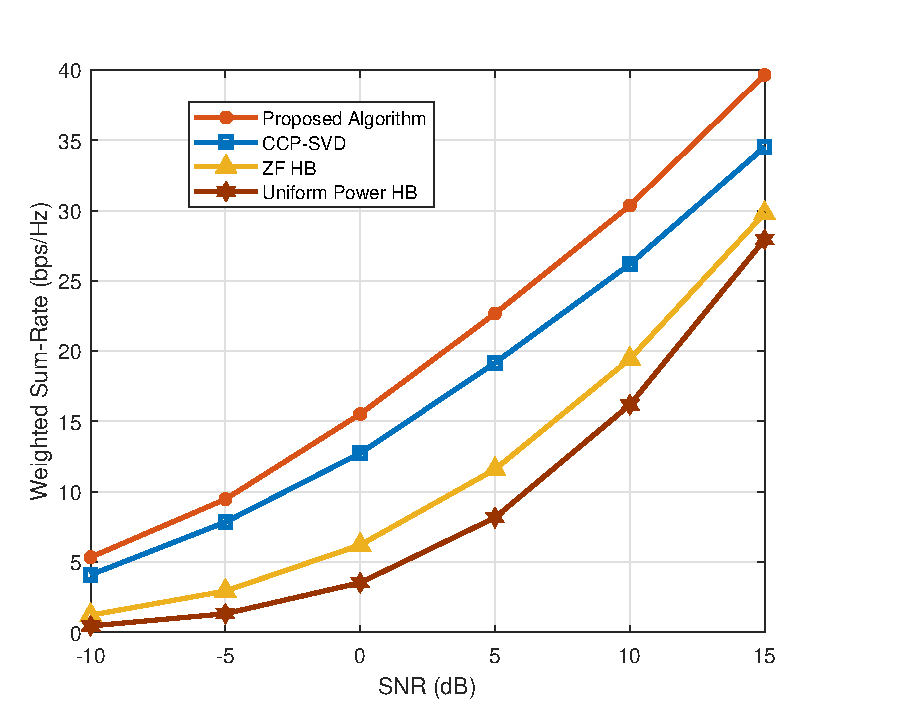
\includegraphics[scale=0.62]{Figure/comparison.eps}
		\caption{Performance comparison for different algorithms.}\label{fig:comparison}
	\end{center}
\end{figure}

Fig.~\ref{fig:cdf} depicts the CDF of the user's data rate. It is evident that all users served by the QoS-aware power allocation algorithms satisfy the minimum QoS requirement (\textit{i.e.} $1$~bps/Hz). In contrast, the conventional zero-forcing algorithm with uniform power allocation suffers from an outage rate of about $20\%$ where the outage is defined as the user data rate being below the minimum required data rate.
\begin{figure}[ht]
	\begin{center}
		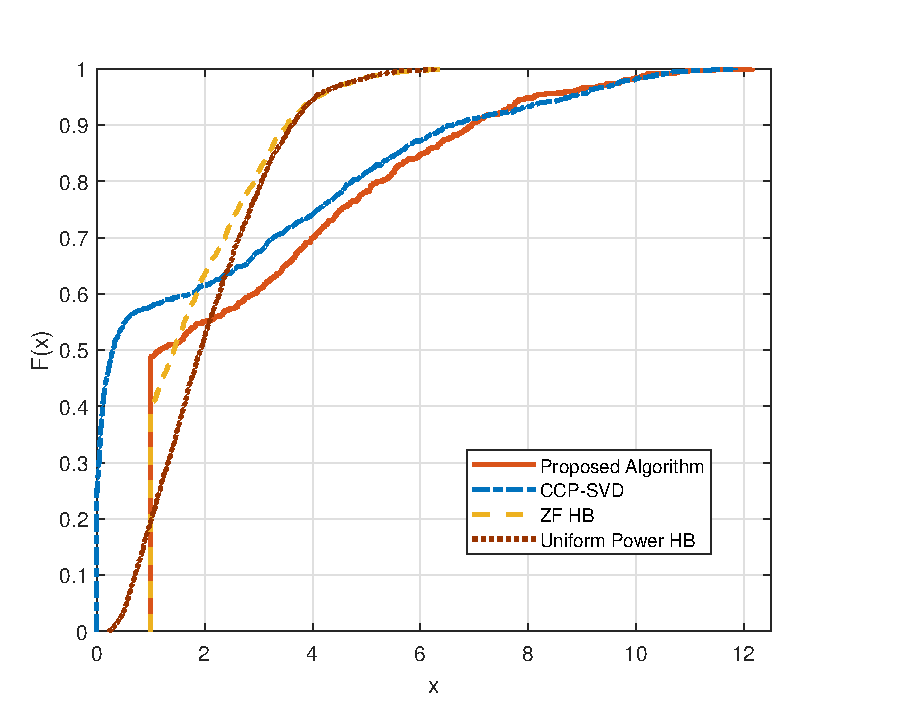
\includegraphics[scale=0.62]{Figure/cdf12users.eps}
		\caption{CDF of users for different algorithms with SNR = $10$ dB.}\label{fig:cdf}
	\end{center}
\end{figure}

%
%Fig. \ref{fig:CDF} compares the CDF of capacities between zero-forcing and proposed algorithm. The additive Gaussian noise is set as $-10$ dB. The figure confirms $C_5$ constraint in $P_1$ as the threshold $\lambda_{u} = 5 $ bps/Hz.
%
%\begin{figure}[ht]
%	\begin{center}
%		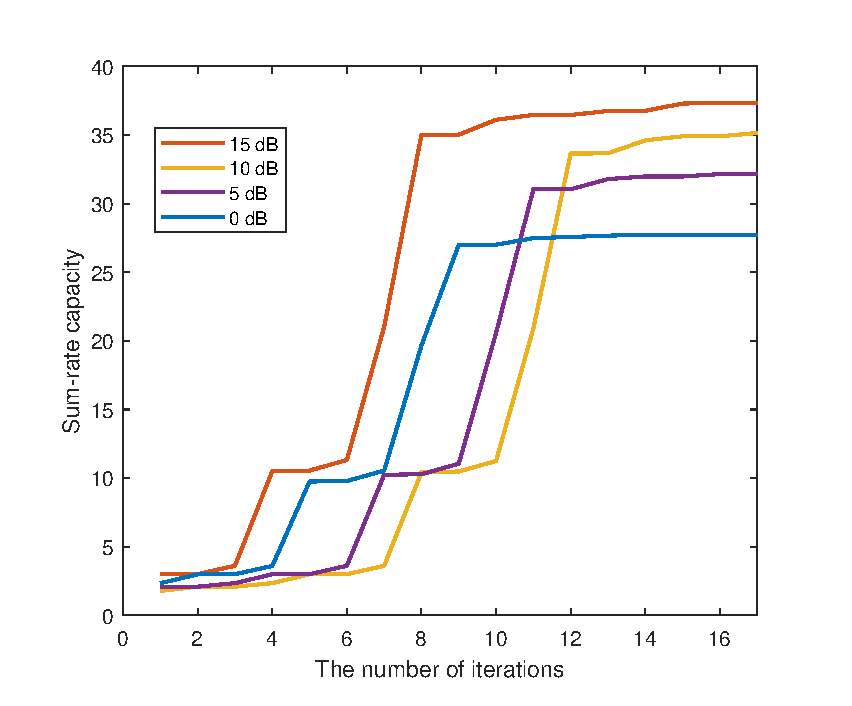
\includegraphics[width=3.5in]{Figure/convergence.eps}
%		\caption{The proof of convergence and monotonicity.}\label{fig:mono}
%	\end{center}
%\end{figure}
%
%Next, the monotonicity and convergence of the proposed iterative algorithm are shown in Fig. \ref{fig:mono} for different given SNR from $0-15$ dB.

\section{Conclusion}
In this paper, we present an algorithm to jointly optimize the digital precoder and power allocation for QoS-aware WSR maximization in the hybrid BDMA transmission systems. To solve the coupled non-convex problem, we first derive the analog precoder by exhaustive searching. Then a rank-constrained D.C. problem is developed. To address the challenge of rank constraint, we propose an iterative algorithm by combining the conventional D.C. problem with RCOP. Finally, the simulation results are given to confirm the effectiveness of the proposed algorithm.

\bibliography{REFDCprecode}
\bibliographystyle{IEEEtran}


%\EOD

\end{document}
